\documentclass[a4paper,titlepage]{ltjsarticle}
\usepackage{graphicx, color, xcolor}
\usepackage{ascmac}
\usepackage{float}
\usepackage{enumitem}
\usepackage{tabularray}
\usepackage{listings}
\usepackage{amssymb}
\usepackage{wrapfig}
\usepackage{diagbox}
\usepackage{siunitx}

\lstset{
    basicstyle=\ttfamily,
    frame=single,
    breaklines=true,
    numbers=left,
    numberstyle=\tiny,
    stepnumber=1,
    numbersep=5pt,
    tabsize=2,
    captionpos=b,
    keywordstyle=\color{blue},
    commentstyle=\color{green!60!black},
    stringstyle=\color{red},
    showstringspaces=false,
    language=VHDL
}

\renewcommand{\thesubsubsection}{・}
\title{情報科学演習C\\
レポート課題1
}
\author{
担当教員\\
\\
\\
\\
\\
基礎工学部 情報科学科 植村向陽\\
学籍番号: 09B24008\\
メールアドレス: u247660i@ecs.osaka-u.ac.jp
}
\date{提出日:\today}
\begin{document}
\maketitle
\section{課題1-1}
\subsection{pingコマンド}
\verb|ping|コマンドは


\begin{verbatim}
$ ping exp001
\end{verbatim}
を実行したところ，以下のような結果が表示された．
\begin{figure}[H]
    \centering
    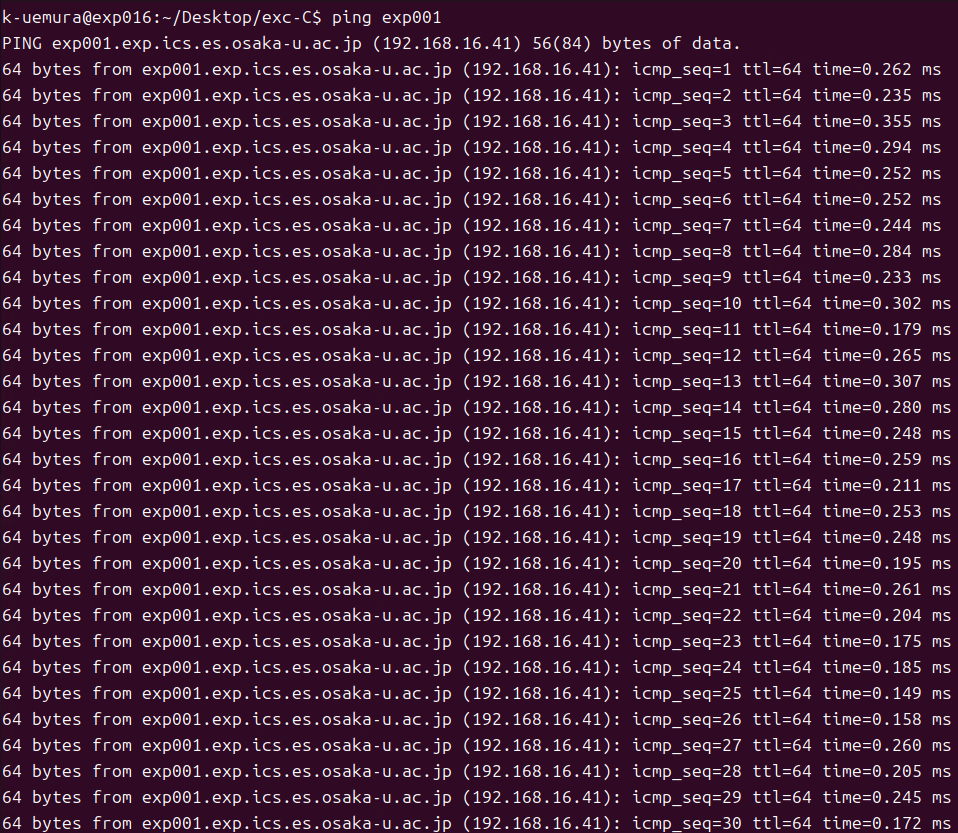
\includegraphics[scale = 0.6]{ping.png}
    \caption{pingコマンドの実行結果}
\end{figure}

\subsection{}
\verb|https://www.osaka-u.ac.jp/ |と \verb| https:
//133.1.138.1/ |をブラウザで開いたところ
どちらも以下のように大阪大学のトップページが表示されたそのため

\subsection{}
\verb|nslookup|コマンドはドメイン名をIPアドレスに変換するか、その逆を行うためのコマンドである．

\section{課題1-2}
\subsection{}

\section{課題1-3}

\end{document}